\item \points{2c} {\bf Degree-$k$ polynomial regression}

Now we extend the idea above to degree-$k$ polynomials by considering $\phi:\mathbb{R}\rightarrow \mathbb{R}^{k+1}$ to be 
		\begin{align}
	\phi(x) = \left[\begin{array}{c} 1\\ x \\ x^2\\ \vdots \\x^k \end{array}\right]\in \mathbb{R}^{k+1} \label{eqn:feature-k}
	\end{align}

Ensure your code from the previous sub-question works with a general $k$.  We will use $k=1,2,3,5,10,20$ as test cases. To verify a correct implementation, autograder test case |2c-7-basic| will create a plot in |src/large-poly.png|.  This plot should look similar to the following:
\begin{figure}[H]
  \centering
  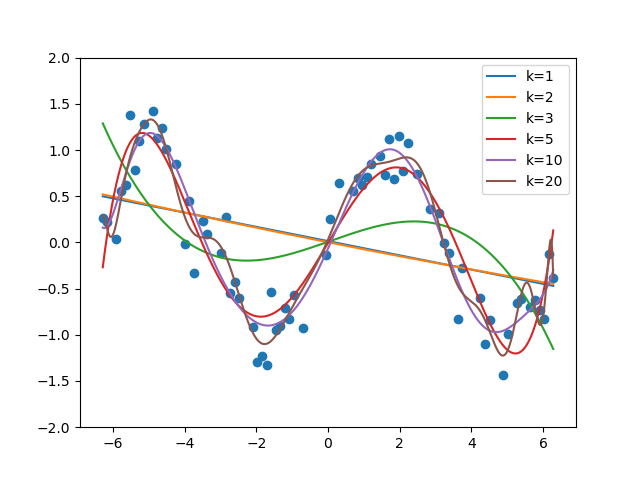
\includegraphics[width=0.65\linewidth]{02-featuremaps/large-poly.png}
  \centering
\caption{Polynomial regression with kernel sizes 1,2,3,5,10 and 20}
\end{figure}
